\documentclass{article}
\usepackage{polski} %moze wymagac dokonfigurowania latexa, ale jest lepszy niż standardowy babel'owy [polish]
\usepackage[utf8]{inputenc}
\usepackage[OT4]{fontenc}
\usepackage{amstext,subcaption,graphicx,color} %include pdf's (and png's for raster graphics... avoid raster graphics!)
\usepackage{url}
\usepackage[pdftex,hyperfootnotes=false,pdfborder={0 0 0}]{hyperref} %za wszystkimi pakietami; pdfborder nie wszedzie tak samo zaimplementowane bo specyfikacja nieprecyzyjna; pod miktex'em po prostu nie widac wtedy ramek


% Zmiana rozmiarów strony tekstu
\addtolength{\voffset}{-1cm}
\addtolength{\hoffset}{-1cm}
\addtolength{\textwidth}{2cm}
\addtolength{\textheight}{2cm}

%bardziej zyciowe parametry sterujace rozmieszczeniem rysunkow
\renewcommand{\topfraction}{.85}
\renewcommand{\bottomfraction}{.7}
\renewcommand{\textfraction}{.15}
\renewcommand{\floatpagefraction}{.66}
\renewcommand{\dbltopfraction}{.66}
\renewcommand{\dblfloatpagefraction}{.66}
\setcounter{topnumber}{9}
\setcounter{bottomnumber}{9}
\setcounter{totalnumber}{20}
\setcounter{dbltopnumber}{9}

% własny bullet list z malymi odstepami
\newenvironment{tightlist}{
\begin{itemize}
  \setlength{\itemsep}{1pt}
  \setlength{\parskip}{0pt}
  \setlength{\parsep}{0pt}}
{\end{itemize}}

%obrazkow szukamy w nastepujacym katalogu:
\graphicspath{{pics/}}



\begin{document}

\thispagestyle{empty} %bez numeru strony

\begin{center}
{\large{Sprawozdanie z laboratorium:\\
Komunikacja człowiek-komputer\\
}}

\vspace{3ex}

Część I: Python i wizualizacja

\vspace{3ex}
{\footnotesize\today}

\end{center}


\vspace{10ex}

Prowadzący: dr hab.~inż. Maciej Komosiński

\vspace{5ex}

Autor:
\begin{tabular}{lllr}
\textbf{Michał Lewiński} & inf122505 & WI & michal.lewinski@student.put.poznan.pl \\
\end{tabular}

\vspace{5ex}

Zajęcia środowe, 16:50.

\vspace{35ex}

\noindent Oświadczam/y, że niniejsze sprawozdanie zostało przygotowane wyłącznie przez powyższych autora/ów,
a wszystkie elementy pochodzące z innych źródeł zostały odpowiednio zaznaczone i~są cytowane w bibliografii.

\newpage


\section{Wstęp}
Zadanie laboratoryjne polegało na utworzeniu gradientów w różnych modelach kolorów oraz zapoznaniu się z wizualizacją wartości skalarnych poprzez mapę z podanymi wysokościami terenu.
\section{Gradienty RGB i HSV}
\begin{figure}
	\begin{subfigure}{0.5\textwidth}
		\begin{center}
			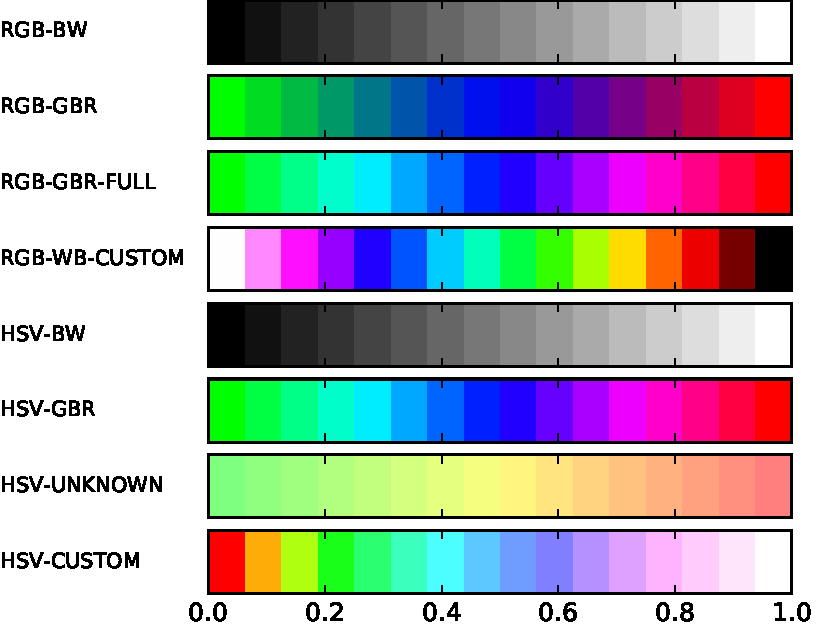
\includegraphics[width=\textwidth]{my-gradients16.pdf}
		\end{center}
	\end{subfigure}
	\begin{subfigure}{0.5\textwidth}
		\begin{center}
			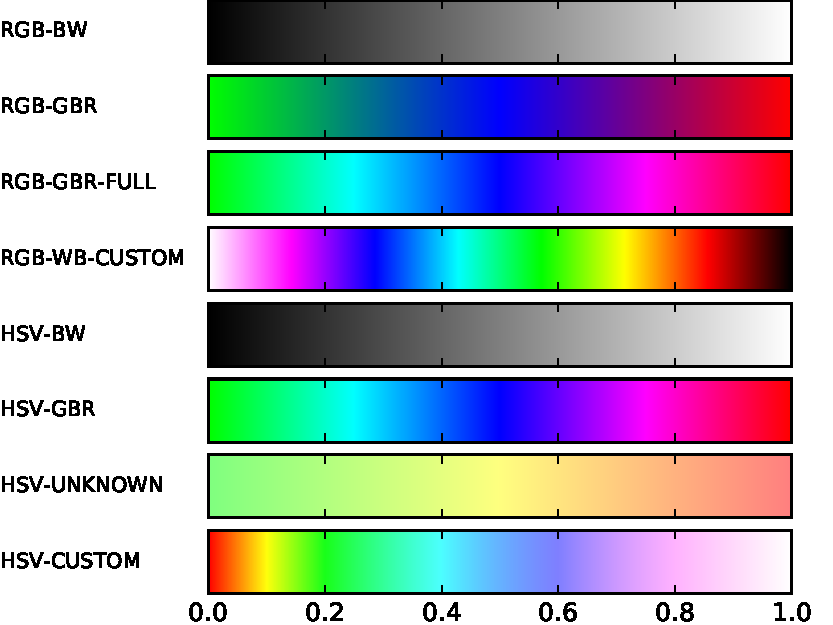
\includegraphics[width=\textwidth]{my-gradients1024.pdf}	
		\end{center}
	\end{subfigure}		
\caption{Gradienty dla 16 i 1042 próbek, bez interpolacji}
\label{fig:gradienty}
\end{figure}
Pierwszym celem zadania było utworzenie 8 gradientów - 4 w modelu RGB oraz 4 pozostałych w modelu HSV. W celu określenia odpowiedniej barwy utworzono funkcję, która dla różnych wartości kolorów zwracała punkt w przestrzeni zależnej od modelu. Dla przestrzeni RGB, funkcja zwracała punkt na ścieżce w sześcianie, natomiast dla HSV w stożku, gdzie \mbox{\(H - \text{odcień}  \in <0,360>, S - \text{nasycenie} \in <0,1>, V - \text{jasność} \in <0,1> \)}. Ponadto, aby wyświetlić barwy w przestrzeni HSV, stworzono funkcję konwertującą model HSV na model RGB. Zamiana polega na wpisaniu stożka w sześcian, gdzie H to kąt w podstawie stożka, S to promień a V to wysokość~\cite{wiki}.  
\newpage
\section{Mapy}
\begin{figure}
	\begin{subfigure}{0.5\textwidth}
			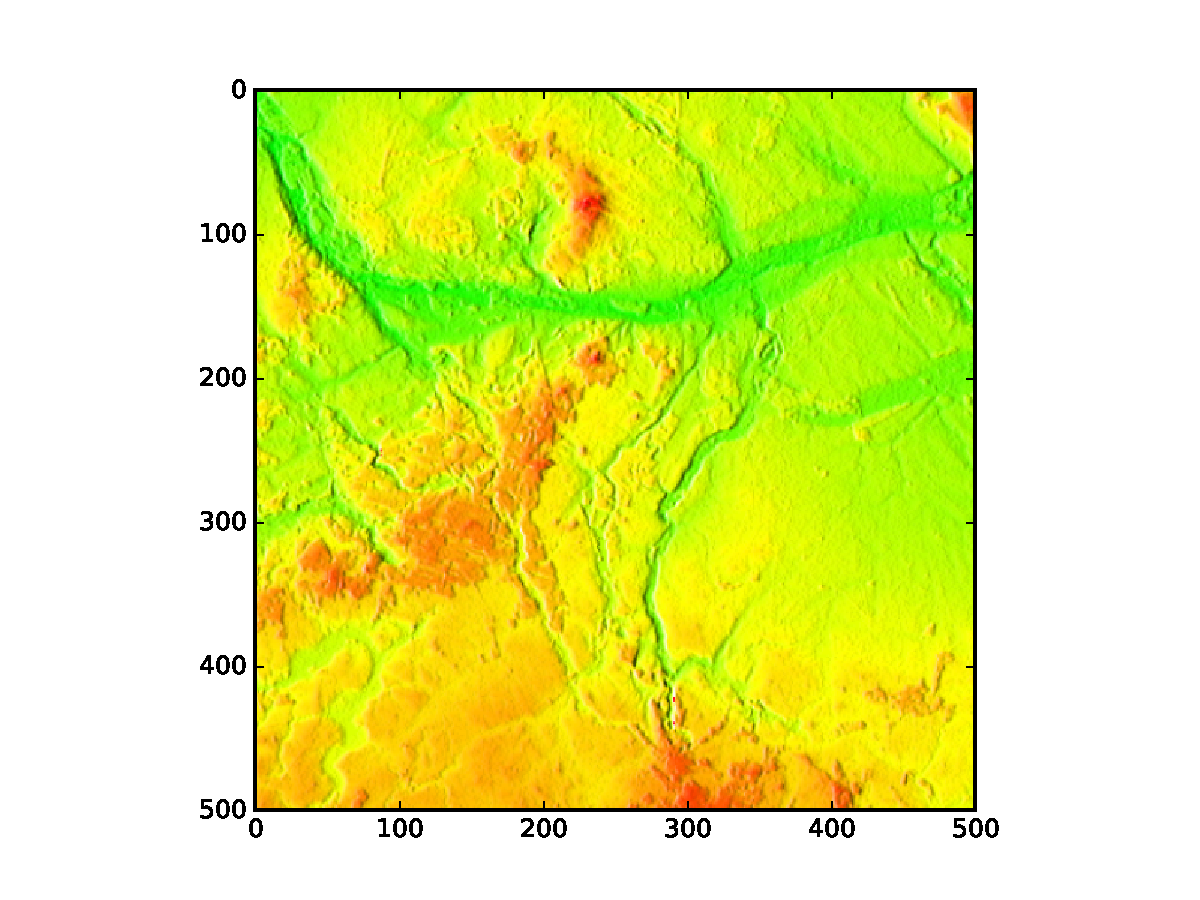
\includegraphics[width=\textwidth]{simpleMap.pdf}
	\end{subfigure}
	\begin{subfigure}{0.5\textwidth}
			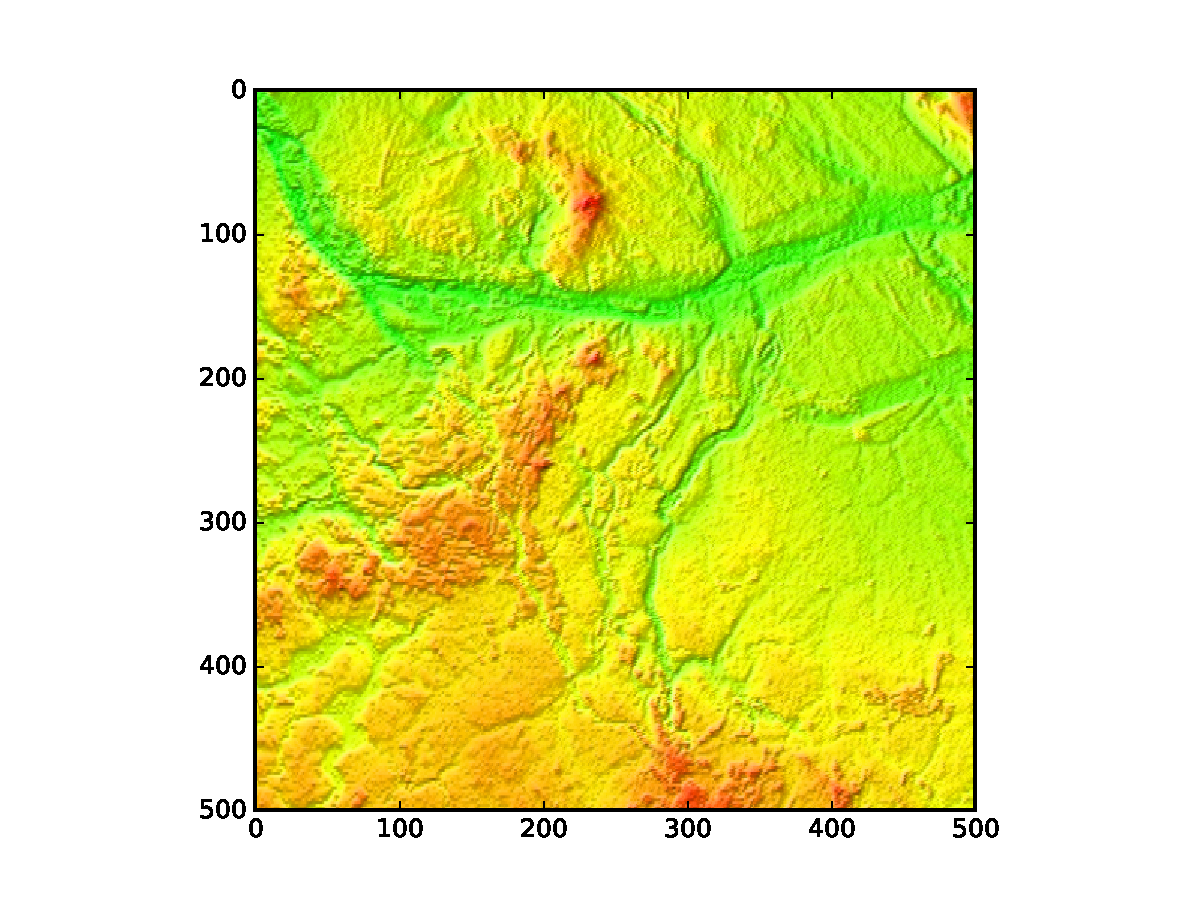
\includegraphics[width=\textwidth]{vectorMap.pdf}	
	\end{subfigure}		
\caption{Wizualizacja mapy terenu przy użyciu prostego i wektorowego algorytmu cieniowania}
\label{fig:mapy}
\end{figure}
Drugim zadaniem była wizualizacja mapy terenu na podstawie pliku z wysokościami. Wykorzystano w tym celu model HSV, gdzie odcień koloru obliczany był na podstawie różnicy wysokości, a następnie ta wartość była znormalizowana do zakresu \mbox{\(<0,120>\)}. Aby poprawić obraz, posłużono się dwoma różnymi algorytmami cieniującymi. Pierwszy algorytm polegał na obliczeniu różnicy wysokości pomiędzy punktem a jego lewym sąsiadem, a następnie odpowiednim przekształcaniu współczynników S i V. Drugi algorytm polegał na obliczeniu kąta pomiędzy wektorem słońca a wektorem normalnym powierzchni. Wektor normalny obliczany był na podstawie iloczynu skalarnego dwóch wektorów, utworzonych z trzech sąsiadujących ze sobą punktów tworzących trójkąt. Otrzymany kąt posłużył do określenia nasycenia i jasności koloru.

\bibliographystyle{plain}
\bibliography{sprawozd}{}

\end{document}
